\documentclass[12pt,fleqn]{article}

\usepackage[utf8]{inputenc}
\usepackage[T2A]{fontenc}
\usepackage[russian]{babel}
\usepackage{graphicx}
\usepackage[footnotesize]{caption2}
\usepackage{indentfirst}
\usepackage{titlesec}

% Параметры страницы
\textheight=24cm
\textwidth=16cm
\oddsidemargin=5mm
\evensidemargin=-5mm
\marginparwidth=36pt
\topmargin=-1cm
\footnotesep=3ex
%\flushbottom
\raggedbottom
\tolerance 3000
% подавить эффект "висячих стpок"
\clubpenalty=10000
\widowpenalty=10000
\renewcommand{\baselinestretch}{1.1}
\renewcommand{\baselinestretch}{1.5} %для печати с большим интервалом
\newcommand{\sectionbreak}{\clearpage}



\begin{document}
\sloppy
	
\begin{titlepage}
\newpage
		
\begin{figure}[t]
	\centering
	
\includegraphics[width=0.4\textwidth]{img/mgu}
\end{figure}
		
\begin{center}
Московский государственный университет имени М.В. Ломоносова \\
Факультет вычислительной математики и кибернетики \\
Кафедра автоматизации систем вычислительных комплексов \\
\end{center}
		
\vspace{6em}
\begin{center}
\large
Ермакова Татьяна Ивановна
\end{center}
		
\begin{center}
\Large
\bfseries
Метод и средства передачи данных в реальном времени в программно-конфигурируемых сетях
\end{center}

\begin{center}
\large
\textsc{
	выпускная квалификационная работа
}
\end{center}

\vspace{4em}
\begin{flushright}
	\textbf{Научный руководитель:}\\
	к.ф.-м.н с.н.с\\
	В.В.Балашов\\
\end{flushright}%


\vspace{\fill}
\begin{center}
Москва 2019
\end{center}
		
\end{titlepage}


\renewcommand{\contentsname}{Содержание}
\tableofcontents

\section*{Введение}
\addcontentsline{toc}{section}{Введение}
текст

\section{Постановка задачи}


\section{Управление трафиком в ВС реального времени с использованием виртуальных каналов}
\subsection{Схема управления трафиком}
\subsection{Реализации схемы управления трафиком}
\subsection{Сравнение реализаций по критерию поддержки реконфигурируемости}


\section{Актуальность задачи}


\section{Алгоритм реконфигурации систем виртуальных каналов}
\subsection{Общая схема алгоритма}
\subsection{Процедуры поиска нового маршрута виртуального канала}
\subsection{Описание базового этапа алгоритма}
\subsection{Описание дополнительного этапа алгоритма}


\section{Структура и функции приложения реконфигурации}
\subsection{Структура приложения реконфигурации}
\subsection{Описание функций служебной части}
\subsection{Описание функций управляющей части}
\subsection{Описание функций монитора}


\section{Программная реализация}
\subsection{Выбор базового программного обеспечения сети}
\subsection{Структура программного средства}
текст

\section{Экспериментальное исследование}
\subsection{Цель исследования}
Целью исследования является подтверждение характеристик предложенного в работе алгоритма реконфигурации систем виртуальных каналов, предназначенного для использования в рамках описанного подхода к передаче данных в ПКС в условиях реального времени. Для достижения поставленной цели необходимо:
\begin{itemize}
	\item провести исследование свойств алгоритма на различных классах входных данных; 
	\item провести апробацию работы алгоритма в составе приложения реконфигурации.
\end{itemize}

Свойства алгоритма, подлежащие исследованию:
\begin{itemize}
	\item успешность и этап завершения;
	\item скорость работы.
\end{itemize}

Изучаемые в рамках апробации подхода характеристики системы:
\begin{itemize}
	\item успешность восстановления трафика в сети после завершения работы алгоритма реконфигурации;
	\item скорость применения изменений в сети;
	\item характеристики качества обслуживания для трафика абонентов.
\end{itemize}

\subsection{Классы исходных данных}
Параметры для формирования классов данных:
\begin{enumerate}
	\item Распределение каналов по пропускным способностям.
	\item Общая загруженность сети.
	\item Топология сети.
\end{enumerate}

Расчёт пропускной способности виртуального канала производится в соответствии с формулой:
$$bw = \frac{LM}{BAG}$$

Выделим три типа виртуальных каналов на основе пропускной способности:
\begin{itemize}
	\item легковесные ($bw=k$);
	\item средние ($bw=2k$);
	\item тяжёлые ($bw=4k$).
\end{itemize}

Классы исходных данных сформированы на основе процентного содержания виртуальных каналов каждого типа и показаны в таблице~\ref{table:bwclass}. Данные классы выбраны для исследования случаев преобладания каждого из типов виртуальных каналов. Распределение пропускных способностей входных потоков данных влияет на работу алгоритма, так как поиск альтернативного маршрута для виртуальных каналов затрудняется с ростом их пропускной способности.

\begin{table}[h]
\begin{center}
\begin{tabular}{|c|c|c|c|}
\hline
	  & Легковесные & Средние & Тяжёлые\\
\hline
	1 & 90\% & 7\% & 3\% \\
\hline
    2 & 10\% & 80\% & 10\% \\
\hline
	3 & 33\% & 34\% & 33\% \\
\hline
	4 & 5\% & 15\% & 80\% \\
\hline
\end{tabular}
\end{center}
\caption{Классы данных на основе пропускной способности}
\label{table:bwclass}
\end{table}

Расчёт общей загруженности сети производится при помощи формулы, отражающей утилизацию физических линий в зависимости от количества маршрутов виртуальных каналов, которые могут быть проложены через данную линию.

Для графа сети, в котором ребра соответствуют физическим линиям, введём вес ребра $e$:
$$p_{e} = \sum_{vl}\frac{bw_{vl} \ast k_{vl_e}}{k_{vl}}$$
где 
\begin{itemize}
	\item $vl$ -- множество виртуальных каналов;
	\item $bw_{vl}$ -- пропускная способность виртуального канала;
	\item $k_{vl_e}$ -- число кратчайших путей, построенных для данного канала, проходящих через это ребро;
	\item $k_{vl}$ -- количество найденных кратчайших путей для данного виртуального канала.
\end{itemize}

Тогда общая загруженность сети определяется формулой:
$$p = \max_{e}\frac{p_{e}}{bw_{e}}$$

где $bw_{e}$ -- пропускная способность физической линии.

Два класса исходных данных, формирующиеся на основе данного параметра, показаны в таблице~\ref{table:loadclass}. Общая загруженность сети влияет на работу исследуемого алгоритма. С ростом загруженности возрастает сложность поиска альтернативных маршрутов для виртуальных каналов. 

\begin{table}[h]
\begin{center}
\begin{tabular}{|c|c|}
\hline
	& Загруженность сети ($p$)\\
\hline
	1 & 60\% \\
\hline
	2 & 80\%  \\
\hline
\end{tabular}
\end{center}
\caption{Классы данных на основе загруженности сети}
\label{table:loadclass}`
\end{table}

Для демонстрации различных случаев поиска альтернативного маршрута и апробации выхода из строя различных элементов сети было выбрано три топологии:
\begin{enumerate}
	\item <<Ромб>> -- позволяет исследовать базовые поломки (Рис.~\ref{pic:4node}).
	\item <<Двойное резервирование>> -- позволяет исследовать выход из строя линий, соединяющих абонентов с коммутаторами (Рис.~\ref{pic:double}).
	\item <<add Название>> -- позволяет исследовать выход из строя коммутатора (Рис.~\ref{pic:5node}).
\end{enumerate}

\begin{figure}[h!]
	\centering
	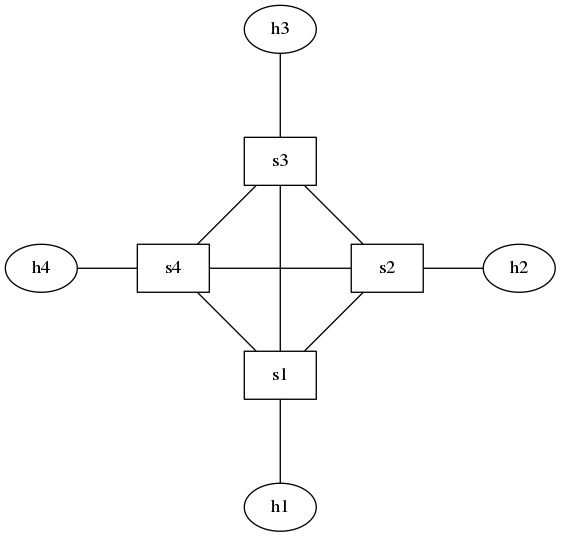
\includegraphics[width=0.40\textwidth]{img/4node.png}
	\caption{Топология <<Ромб>>.}
	\label{pic:4node}
\end{figure}

\begin{figure}[h!]
	\centering
	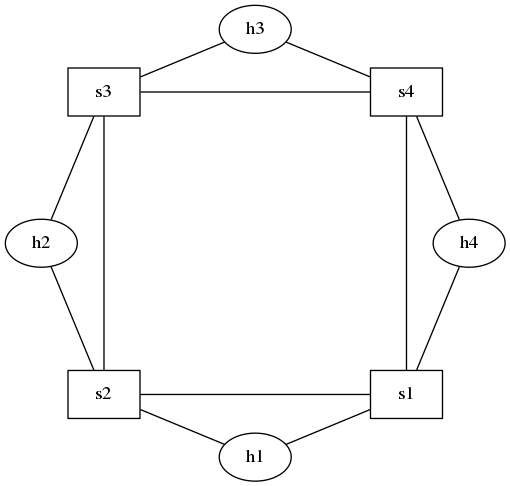
\includegraphics[width=0.40\textwidth]{img/double.png}
	\caption[russian]{Топология <<Двойное резервирование>>.}
	\label{pic:double}
\end{figure}

\begin{figure}[h!]
	\centering
	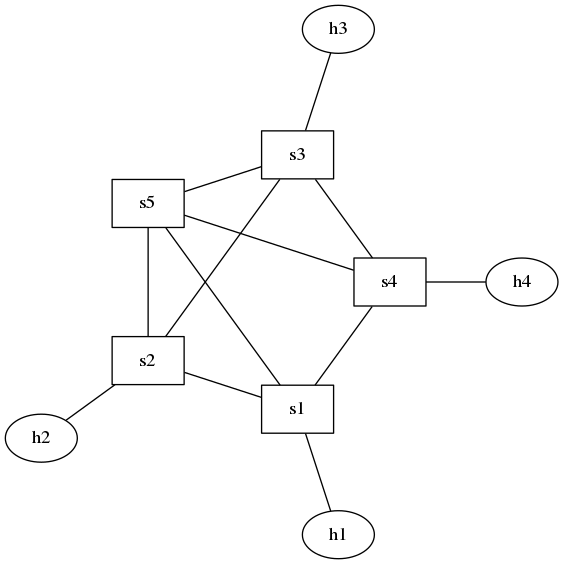
\includegraphics[width=0.40\textwidth]{img/5node.png}
	\caption{Топология <<add Название>>.}
	\label{pic:5node}
\end{figure}

В исследовании используется рекомендованное экспертами в области вычислительных систем реального времени число потоков данных равное 100.

\subsection{Исследование свойств алгоритма}
\subsubsection{Методика исследования}

\subsubsection{Результаты}
Характеристики компьютера, на котором производилось исследование:
\begin{itemize}
	\item Процессор -- Intel Core i7, тактовая частота 1.90 ГГц.
	\item Оперативная память -- 4 ГБ.
\end{itemize}

Результаты исследования свойств алгоритма реконфигурации систем виртуальных каналов приведены ниже в addПриложение (см. таблицу addТаблица).

Максимальное время работы алгоритма – addмс. Данные показатели времени достигаются, если алгоритм вынужден выполнить дополнительный этап. Следует отметить, что выполнение дополнительного этапа произошло в add\% случаев. Как правило алгоритм завершает работу на базовом этапе. При таком варианте выполнения время завершения алгоритма не превышает addмс.

Алгоритм не смог построить новую систему виртуальных каналов при add. Это объясняется тем, что add.

add Возможно стоит сказать что-то о соотношении времени работы алгоритма и задержек в сети чтобы знать почему это нормально. Может типовые периоды сообщений?

\subsection{Апробация разработанного подхода динамической реконфигурации сети}
\subsubsection{Конфигурация экспериментальной системы}
Система апробации представляет собой виртуальную среду, имитирующую
функционирование:
\begin{enumerate}
	\item Контроллера сети.
	\item Набора коммутаторов.
	\item Абонентов сети, формирующих потоки данных с заданными характеристиками.
\end{enumerate}

Виртуальная среда разворачивается на основе операционной системы Ubuntu 16.04,
на которой установлены следующие компоненты:
\begin{enumerate}
	\item Runos -- ПКС-контроллер [addlink].
	\item Ofsoftswitch13 -- программный коммутатор, поддерживающий OpenFlow 1.3 [addlink].
	\item Mininet -- средство эмуляции сети [addlink].
\end{enumerate}

\subsubsection{Методика апробации}
\subsubsection{Сценарии апробации}
\subsubsection{Результаты}
\subsection{Выводы}


\section*{Заключение}
\addcontentsline{toc}{section}{Заключение}
текст

\renewcommand{\bibname}{Список литературы}

\end{document}






